% ----------------------------------------------------------------
% Report Class (This is a LaTeX2e document)  *********************
% ----------------------------------------------------------------
\documentclass[11pt]{article}
\usepackage[english]{babel}
\usepackage{amsmath,amsthm}
\usepackage{amsfonts}
\usepackage{fancyhdr}
\usepackage{graphicx,xcolor}
\usepackage{geometry,cite}
\fancyhead{}
\fancyfoot{}
\fancyhead[L]{\footnotesize{\textsf{Alex Cutforth | 24375019}}}
\fancyhead[R]{\footnotesize{\textsf{ENME 203, Project 2025, \today}}}
\fancyfoot[R]{\footnotesize{\textsf{page \thepage}}}
\geometry{ %showframe,               % shows frame, helpful for initial setup
           includehead,              % header
           includefoot,              % footer                "
           paper       = a4paper,    % paper format
           top         = 2.0 cm,     % margin top
           bottom      = 1.0 cm,     % margin bottom
           inner       = 2.0 cm,     % margin left (inner if "twoside")
           outer       = 2.0 cm,     % margin right (outer if "twoside")
           headheight  = 0.5 cm,     % space headline
           headsep     = 0.5 cm,     % distance header to text
           footskip    = 0.5 cm      % distance text to footer
         }
\pagestyle{fancy}
% ----------------------------------------------------------------
\begin{document}
\begin{titlepage}
\hfill
\includegraphics[width=40mm]{UCLogo.png}
\begin{center}

\vspace*{\fill}

\textbf{\huge{\textsl{Dynamics of a simplified wingsuit}}}\\
ENME203 2025 Project\\
\vspace*{\fill}


\textbf{\large Alex Cutforth}

\textbf{\large acu60@uclive.ac.nz}

\vspace*{\fill}

\textnormal{\large \today}

\end{center}
\end{titlepage}

% ----------------------------------------------------------------
\section*{Abstract}
\textcolor[rgb]{0.80,0.29,0.09}{\textsl{[This space is filled with a brief summary about all of the content of this report. It describes and connects all sections: Include topic, main idea, aims, model and method /types of analyses used, and findings and conclusions. Approximate length: 120 words +/- 10\%.]}}


% ----------------------------------------------------------------
\section*{Introduction}
This project focuses on analysing the properties of a simplified wingsuit model, this includes but is not limited to:
\begin{itemize}
  \item Kinematic analysis of significant points on the wingsuit
  \item Derivation of moments of interia, and relevant equations of motion
  \item Optimization of wingsuit properties for stability improvement
\end{itemize}
\textcolor[rgb]{0.80,0.29,0.09}{\textsl{[The introduction of this technical report includes a bit of background and purpose of the project. Identify the subject, background information on its development and use, the aims of the project’s analyses, and the purpose of the project. A complete literature review is usually part of professional communications, to inform the reader of the current state of the research on the subject. A very brief version of that is appropriate here:}}
\begin{enumerate}
  \item \textcolor[rgb]{0.80,0.29,0.09}{\textsl{Please cite 2-3 sources (no links to websites, e.g. Wikipedia – use scholarly/professional sources) used to inform your writing of this section}}
  \item \textcolor[rgb]{0.80,0.29,0.09}{\textsl{Include all citations in your list of References. The Reference list should be on its own page.}}
  \item \textcolor[rgb]{0.80,0.29,0.09}{\textsl{The IEEE referencing style should be used.}}
  \item \textcolor[rgb]{0.80,0.29,0.09}{\textsl{Approximate length: 150-200 words.}}
\end{enumerate}
\textcolor[rgb]{0.80,0.29,0.09}{\textsl{Example: In this example sentence I refer to one of my own publications on MEMS technology \cite{gutschmidt2024} to make you aware of the IEEE standard \cite{IEEE} which is mostly used for engineering articles and reports. (The work cited here is totally unrelated to the project!)]}}


% ----------------------------------------------------------------
\section*{Model Description}
The wingsuit side profile is based on a symmetric 1m long NACA0012 foil.
However this shape is only relevant for the derivation of Moments and Products of Inertia.\\\\
$k = 1500$ N/m, $k_{\theta} = 200$ Nm/rad, $d = 150$ Ns/m, $d_{\theta} = 0.03$ Nms/rad, $l_{\theta} = 0.1$ m, $l_{\alpha} = 0.05$ m, $m = 2$ kg, $I^F = 0.13$ kgm\textsuperscript{2}, $C_{\theta} = 0.4$ kg/m, $C_y = 0.6$ kg/m
\\\\
\textcolor[rgb]{0.80,0.29,0.09}{\textsl{[In this section, briefly describe the model and underlying assumptions. This includes using figures with figure descriptions and referencing to these in the text.]}}

\begin{figure}[h!]
  \centering
  \caption{...}\label{fig:model}
\end{figure}

% ----------------------------------------------------------------
\section*{Method}\label{sec:method}
\textcolor[rgb]{0.80,0.29,0.09}{\textsl{[This section brings parts 1 and 2 of the project together. Begin with 1-2 sentences explaining the overarching method of using Newton’s/Euler’s method to bring together kinematics (part1) and dynamics (part 2) to generate the EOM.  Include any constraint equations (as part of the analysis, if applicable). Details of the method will then be explained in the following sub-sections: Kinematics, Dynamics and Equations of Motion.]}}


% ----------------------------------------------------------------
\subsection*{Kinematics}\label{sec:kin}
Since the centre of rotation is not in the same place as the centre of mass for this system, it is neccessary to derive kinematic relations between angular velocities/accelerations and relative translational velocities/accelerations.
\begin{align}
  v_{G/F} &=
  \begin{pmatrix}
     \dot{\theta}l_{\theta}\sin\theta \\
    -\dot{\theta}l_{\theta}\cos\theta \\
  \end{pmatrix} \label{eq:kin1} \\
  a_{G/F} &=
  \begin{pmatrix}
     \ddot{\theta}l_{\theta}\sin\theta + \dot{\theta}^2l_{\theta}\cos\theta \\
    -\ddot{\theta}l_{\theta}\cos\theta + \dot{\theta}^2l_{\theta}\sin\theta 
  \end{pmatrix} \label{eq:kin2}
\end{align}
\begin{figure}[h!]
  \centering
  \caption{...}\label{fig:kin_sketch}
\end{figure}

% ----------------------------------------------------------------
\subsection*{Dynamics}\label{sec:dyn}
The equations of motions use the format of the basic translational and rotational mass/dampener/spring systems:
\begin{align*}
  m\ddot{y} + d\dot{y} + ky &= F \\
  I\ddot{\theta} + d_{\theta}\dot{\theta} + k_{\theta}\theta &= T
\end{align*}
The symbols $F$ and $T$ represent external force and torque acting upon the system, which for this model is just the lift force acting at point A
\begin{align*}
  m\ddot{y} + d\dot{y} + ky &= L = C_{\theta}U^2\theta + C_yU\dot{y} \\
  I\ddot{\theta} + d_{\theta}\dot{\theta} + k_{\theta}\theta &= l_{\alpha}\theta = l_{\alpha}(C_{\theta}U^2\theta + C_yU\dot{y})
\end{align*}
Then, since the centre of rotation is not in the same location as the centre of mass, the equations must be linearized, giving the final equations of motion:
\begin{align}
  m\ddot{y} - ml_{\theta}\ddot{\theta} + d\dot{y} + ky &= L = C_{\theta}U^2\theta + C_yU\dot{y}\label{eq:eom1} \\
  I\ddot{\theta} - ml_{\theta}\ddot{y} + d_{\theta}\dot{\theta} + k_{\theta}\theta &= l_{\alpha}\theta = l_{\alpha}(C_{\theta}U^2\theta + C_yU\dot{y})\label{eq:eom2}
\end{align}
This is a 2 degrees of freedom system, hence why there are two seperate equations of motion. This is because the translational and rotational properties of the system are not completely dependent upon each other. However, they are \textsl{partially} dependent, which is why there is sharing of quantities between equations. These are known as coupled equations.

[\textcolor[rgb]{0.80,0.29,0.09}{\textsl{This section mainly contains content of Project Part 2. Introduce the kinetic relations using/referring to a free-body-diagram.}}] 

% ----------------------------------------------------------------
\subsection*{Equation of Motion}\label{sec:eom}
[\textcolor[rgb]{0.80,0.29,0.09}{\textsl{This section mainly contains content of Project Part 2. Briefly describe the derivation of the equation(s) of motion. Explain the degrees of freedom, and any underlying assumptions. Accompany the method with necessary sketches (e.g. free-body diagram(s) etc.).}}]

% ----------------------------------------------------------------
\section*{Analysis \& Discussions}\label{sec:anal_disc}
[\textcolor[rgb]{0.80,0.29,0.09}{\textsl{This section mainly contains content of Project Part 3. Present results professionally by relating figures/graphs to equation numbers, describing graphs and observations, and discussing results and their meaning.]}}
\subsection*{Decoupled Analysis}\label{sec:coupled_analysis}
As stated in the Dynamics section, the equations of motion for this system are coupled, this means the equations can not be analysed induvidually, but rather as a system of differential equations.
However, it is possible to set specific conditions where the equations decouple from each other, this occurs when the centre of mass and flexural axis are aligned ($l_{\theta} = 0$), and the lift coefficient associated with the equation in question's quantity is set to zero ($C_y$ or $C_{\theta} = 0 $). \\\\
Case 1, where $l_{\theta} = 0$ and $C_y = 0$ results in an equation of motion for rotation of
\begin{equation}
  \ddot{\theta}+\frac{d_{\theta}}{I^F}\dot{\theta}+\frac{k_{\theta}-l_{\alpha}C_{\theta}U^2}{I^F}\theta = 0 \label{eq:decoupled1}
\end{equation}
This equation can then be considered with the format $\ddot{q} + 2\zeta\omega\dot{q}+\omega^2q = 0$, giving the formulas for frequency and damping ratio:
\begin{align*}
  \omega &= \sqrt{\frac{k_{\theta}-l_{\alpha}C_{\theta}U^2}{I^F}} \\
  \zeta &= \frac{d_{\theta}}{2\sqrt{I^F(k_{\theta}-l_{\alpha}C_{\theta}U^2)}}
\end{align*}
This information allows us to find a critical airspeed where the wingsuit's torsional mode becomes statically unstable.
This critical airspeed occurs when the real component of the roots (given by $\lambda = -\zeta\omega\pm i\omega\sqrt{1-\zeta^2}$) of the equation of motion equal zero.
Given a positive value for $d_{\theta}$, the equation for $\zeta$ cannot be zero, so to find the solution, $\omega$ must be set to zero. This gives:
\begin{align*}
  k_{\theta} &= l_{\alpha}C_{\theta}U^2 \\
  U &= \sqrt{\frac{k_{\theta}}{l_{\alpha}C_{\theta}}}\\
    &= 100~\mathrm{m/s}
\end{align*}

\subsection*{Modal Analysis}\label{sec:modal_analysis}
Modal analysis allows us to see the stability of the system as a whole when both degrees of freedom are partially interacting.
To analyse both equations of motion simultaneously they can be represented in a matrix system of the form
$$
  \mathbf{M}\ddot{X}+\mathbf{D}\dot{X}+\mathbf{K}X = 0
$$
Then substituting in equations \ref{eq:eom1} and \ref{eq:eom2}
$$
  \overbrace{
    \begin{bmatrix}
      I^F&-ml_{\theta} \\
      -ml_{\theta}&m
    \end{bmatrix}
  }^{\mathbf{M}}
  \overbrace{
    \begin{bmatrix}
      \ddot{\theta} \\
      \ddot{y}
    \end{bmatrix}
  }^{\ddot{X}}
  +
  \overbrace{
    \begin{bmatrix}
      d_{\theta}&-l_{\alpha}C_yU\\
      0&d-C_yU
    \end{bmatrix}
  }^{\mathbf{D}}
  \overbrace{
    \begin{bmatrix}
      \dot{\theta} \\
      \dot{y}
    \end{bmatrix}
  }^{\dot{X}}
  +
  \overbrace{
    \begin{bmatrix}
      k_{\theta}-l_{\alpha}C_{\theta}U^2&0\\
    -C_{\theta}U^2&k
    \end{bmatrix}
  }^{\mathbf{K}}
  \overbrace{
    \begin{bmatrix}
      \theta \\
      y
    \end{bmatrix}
  }^X
  = 0
$$
This system can then be converted into state space
\begin{align*}
  \begin{bmatrix}
    I&0\\
    0&M
  \end{bmatrix}
  \begin{bmatrix}
    \dot{X}\\
    \ddot{X}
  \end{bmatrix}
  +
  \begin{bmatrix}
    0&-I\\
    K&D
  \end{bmatrix}
  \begin{bmatrix}
    X\\
    \dot{X}
  \end{bmatrix}
  &=0
  \\
  \frac{d}{dt}
  \begin{bmatrix}
    X\\
    \dot{X}
  \end{bmatrix}
  &=
  \begin{bmatrix}
    I&0\\
    0&M
  \end{bmatrix}^{-1}
  \begin{bmatrix}
    0&I\\
    -K&-D
  \end{bmatrix}
  \begin{bmatrix}
    X\\
    \dot{X}
  \end{bmatrix}
\end{align*}
This system is suitable for use with an initial value problem numerical solver, and we can analyse the behavior of such a system by finding the eigenvalues of the coefficient matrix
$$
  A = 
  \begin{bmatrix}
    I&0\\
    0&M
  \end{bmatrix}^{-1}
  \begin{bmatrix}
    0&I\\
    -K&-D
  \end{bmatrix}
$$
The roots of this system can then be plotted against Airspeed using an eigenvalue finder. \\
A system is unstable if the real parts of any of its eigenvalues is postive, and Figure \ref{fig:modal_roots} shows that the system has positive real components for approximately $U > 30$ m/s, meaning this wingsuit model is not very stable at the reasonably high speeds needed for flight.
\begin{figure}
  \centering
  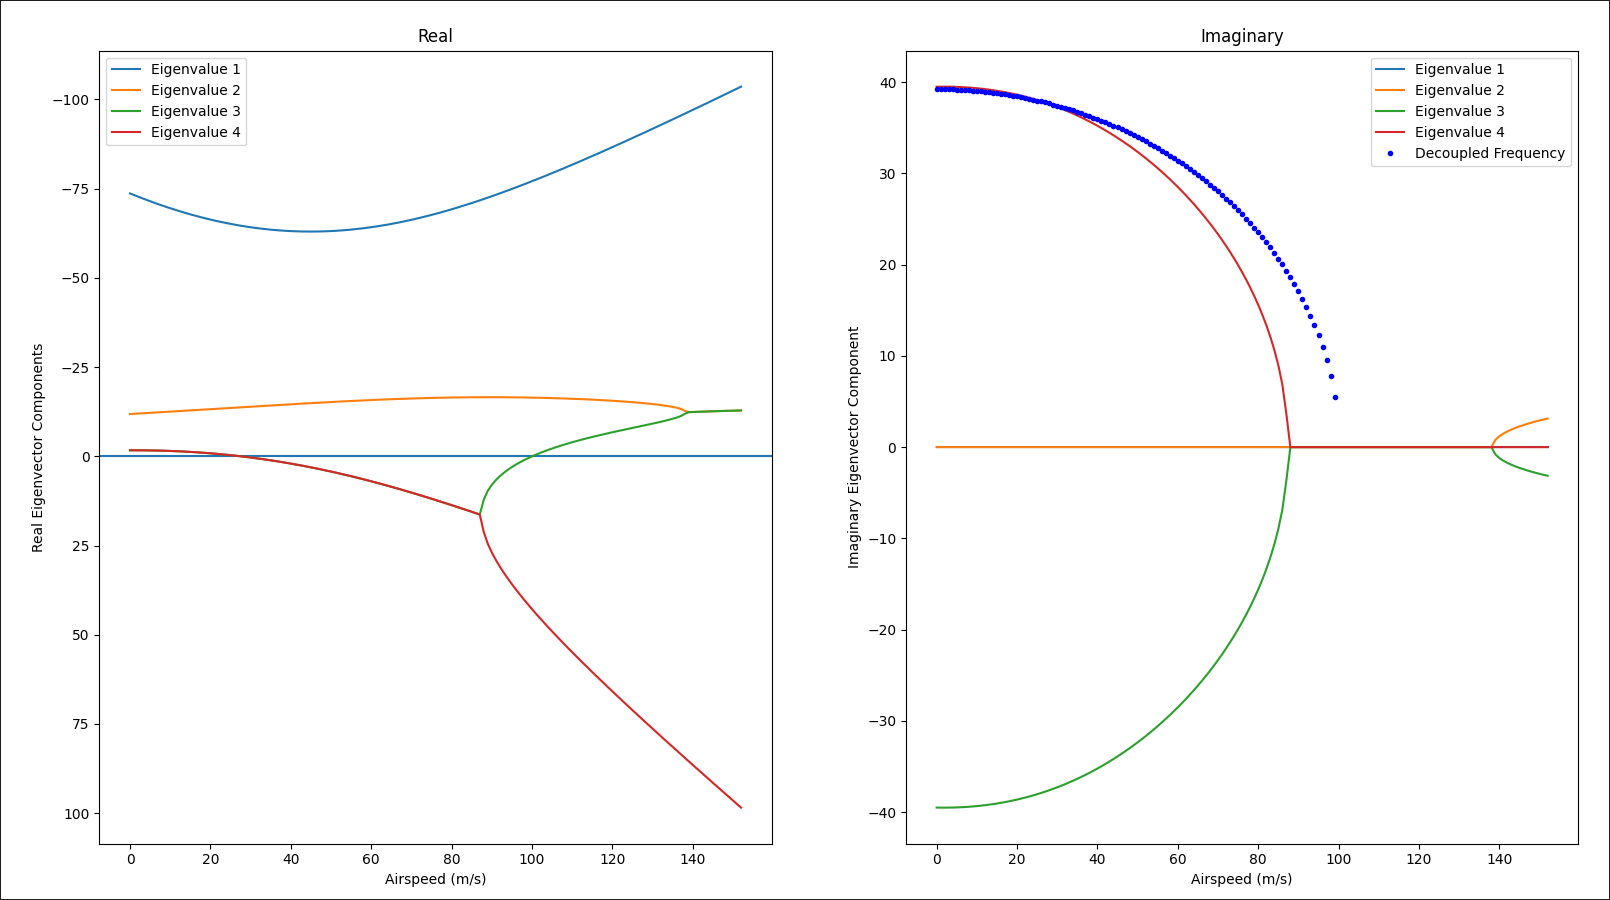
\includegraphics[width=170mm]{modal_roots.png}
  \caption{Modal Roots}\label{fig:modal_roots}
\end{figure}

% ----------------------------------------------------------------
\section*{Conclusions}\label{sec:conclusion}
\textcolor[rgb]{0.80,0.29,0.09}{\textsl{[Wrap up the report by summarising key findings and linking results back to the motivation/purpose of the project as described in Introduction section. Approximate length: 80-120 words]}}


% ----------------------------------------------------------------
\bibliography{project}{}
\bibliographystyle{unsrt}

\end{document}
% ----------------------------------------------------------------
